% Chapter Template

\chapter{The Transmitter} % Main chapter title
\label{Chapter6} 


\section{Introduction}

The transmitter for the sound-based move tracking protocol is in charge
of creating the tones representing each centerpiece's current state,
and updating those tones each time a centerpiece changes state.

This chapter will detail a proof-of-concept design for a printed
circuit board (PCB) capable of generating all the tones required for
encoding one centerpiece's state.

This chapter assumes that the reader has a knowledge of basic circuit
components like resistors and capacitors. It begins with a discussion
of the requirements/constraints for the physical transmitter (Section
\ref{sec:transmitter-requirements}). From there a formal design
schematic for the transmitter will be presented (Section
\ref{sec:transmitter-design}) and prototyped (Sections
\ref{sec:prototype}) followed by an analysis of the effects of the
centercap enclosure on signal strength (Section
\ref{sec:minimizing-sound-obstruction}). Finally, all the required
components for the transmitter will be laid out inside a single
speedcube centercap to demonstrate the viability of the presented
design (Section \ref{sec:miniaturization}).


\section{Requirements}
\label{sec:transmitter-requirements}

This section will detail the constraints within which the transmitter
will be required to operate. These constraints include the precision of
tone generation (Section \ref{subsec:precision-of-tone-generation}),
the reliability of the transmitter in changing tones to reflect a face
turn (Section \ref{subsec:responsiveness-to-face-turns}), the intensity
of output audio that the transmitter can produce (Section
\ref{subsec:transmitter-signal-to-noise-ratio}), and the physical size
of the transmitter (Section \ref{subsec:prospects-of-miniaturization}).

\subsection{Precision of Tone Generation}
\label{subsec:precision-of-tone-generation}

While the receiver specified in Chapter \ref{Chapter5} supports custom
state to frequency mappings, it expects that the frequency
corresponding to each centerpiece's state stays constant throughout the
entire audio recording. As such, the chosen transmitter design can
encode centerpiece states with any frequency (assuming the chosen
frequencies work within the constraints specified in Section
\ref{sec:protocol-requirements}), but it must produce its chosen
frequencies with high precision.

\subsection{Responsiveness to Face Turns}
\label{subsec:responsiveness-to-face-turns}

The chosen transmitter design must respond to an applied face turn by
changing the currently transmitted audio frequency to the frequency
corresponding to the new centerpiece state. Given top speedcubers'
burst turn speeds of 20 TPS (see Section \ref{sec:alternatives}) this
frequency change must complete and stabilize long enough to be
accurately detected within one twentieth of a second (50ms).

\subsection{Signal-to-Noise Ratio}
\label{subsec:transmitter-signal-to-noise-ratio}

The transmitter must create tones loud enough to be easily
distinguished from ambient noise, including the sound of the Rubik's
Cube's own turns. In light of the above requirement for the transmitter
to fit within a center cubie
(\ref{subsec:prospects-of-miniaturization}), this requirement will also
require the transmitter design to consider how to overcome any audio
dampening caused by such an enclosure.

\subsection{Prospects of Miniaturization}
\label{subsec:prospects-of-miniaturization}

The transmitter must be both removable and small enough to fit in the
center cap of each face of a speedcube. This requirement stems from two
sources. First, in contrast to all existing smartcubes, most
non-smartcubes have small, solid cores (Figure
\ref{fig:356-core-closed}) that provide no extra space for the
inclusion of any electronics, but do have a small amount of open space
within their center cubies (Figure \ref{fig:356-core-open}). Second,
the use of a cube with non-removable, embedded electronics violates the
WCA competition regulation 2i \cite{wca-regulations} (See also Section
\ref{subsec:the-rise-of-smart-cubes}).

\begin{figure}[h]
    \centering
    \caption{Internal pieces of a standard speedcube (Gans 356)}
    \label{fig:356-core}
    \begin{subfigure}{.45\textwidth}
        \centering
        \caption{View of the small, solid plastic core}
        \label{fig:356-core-closed}
        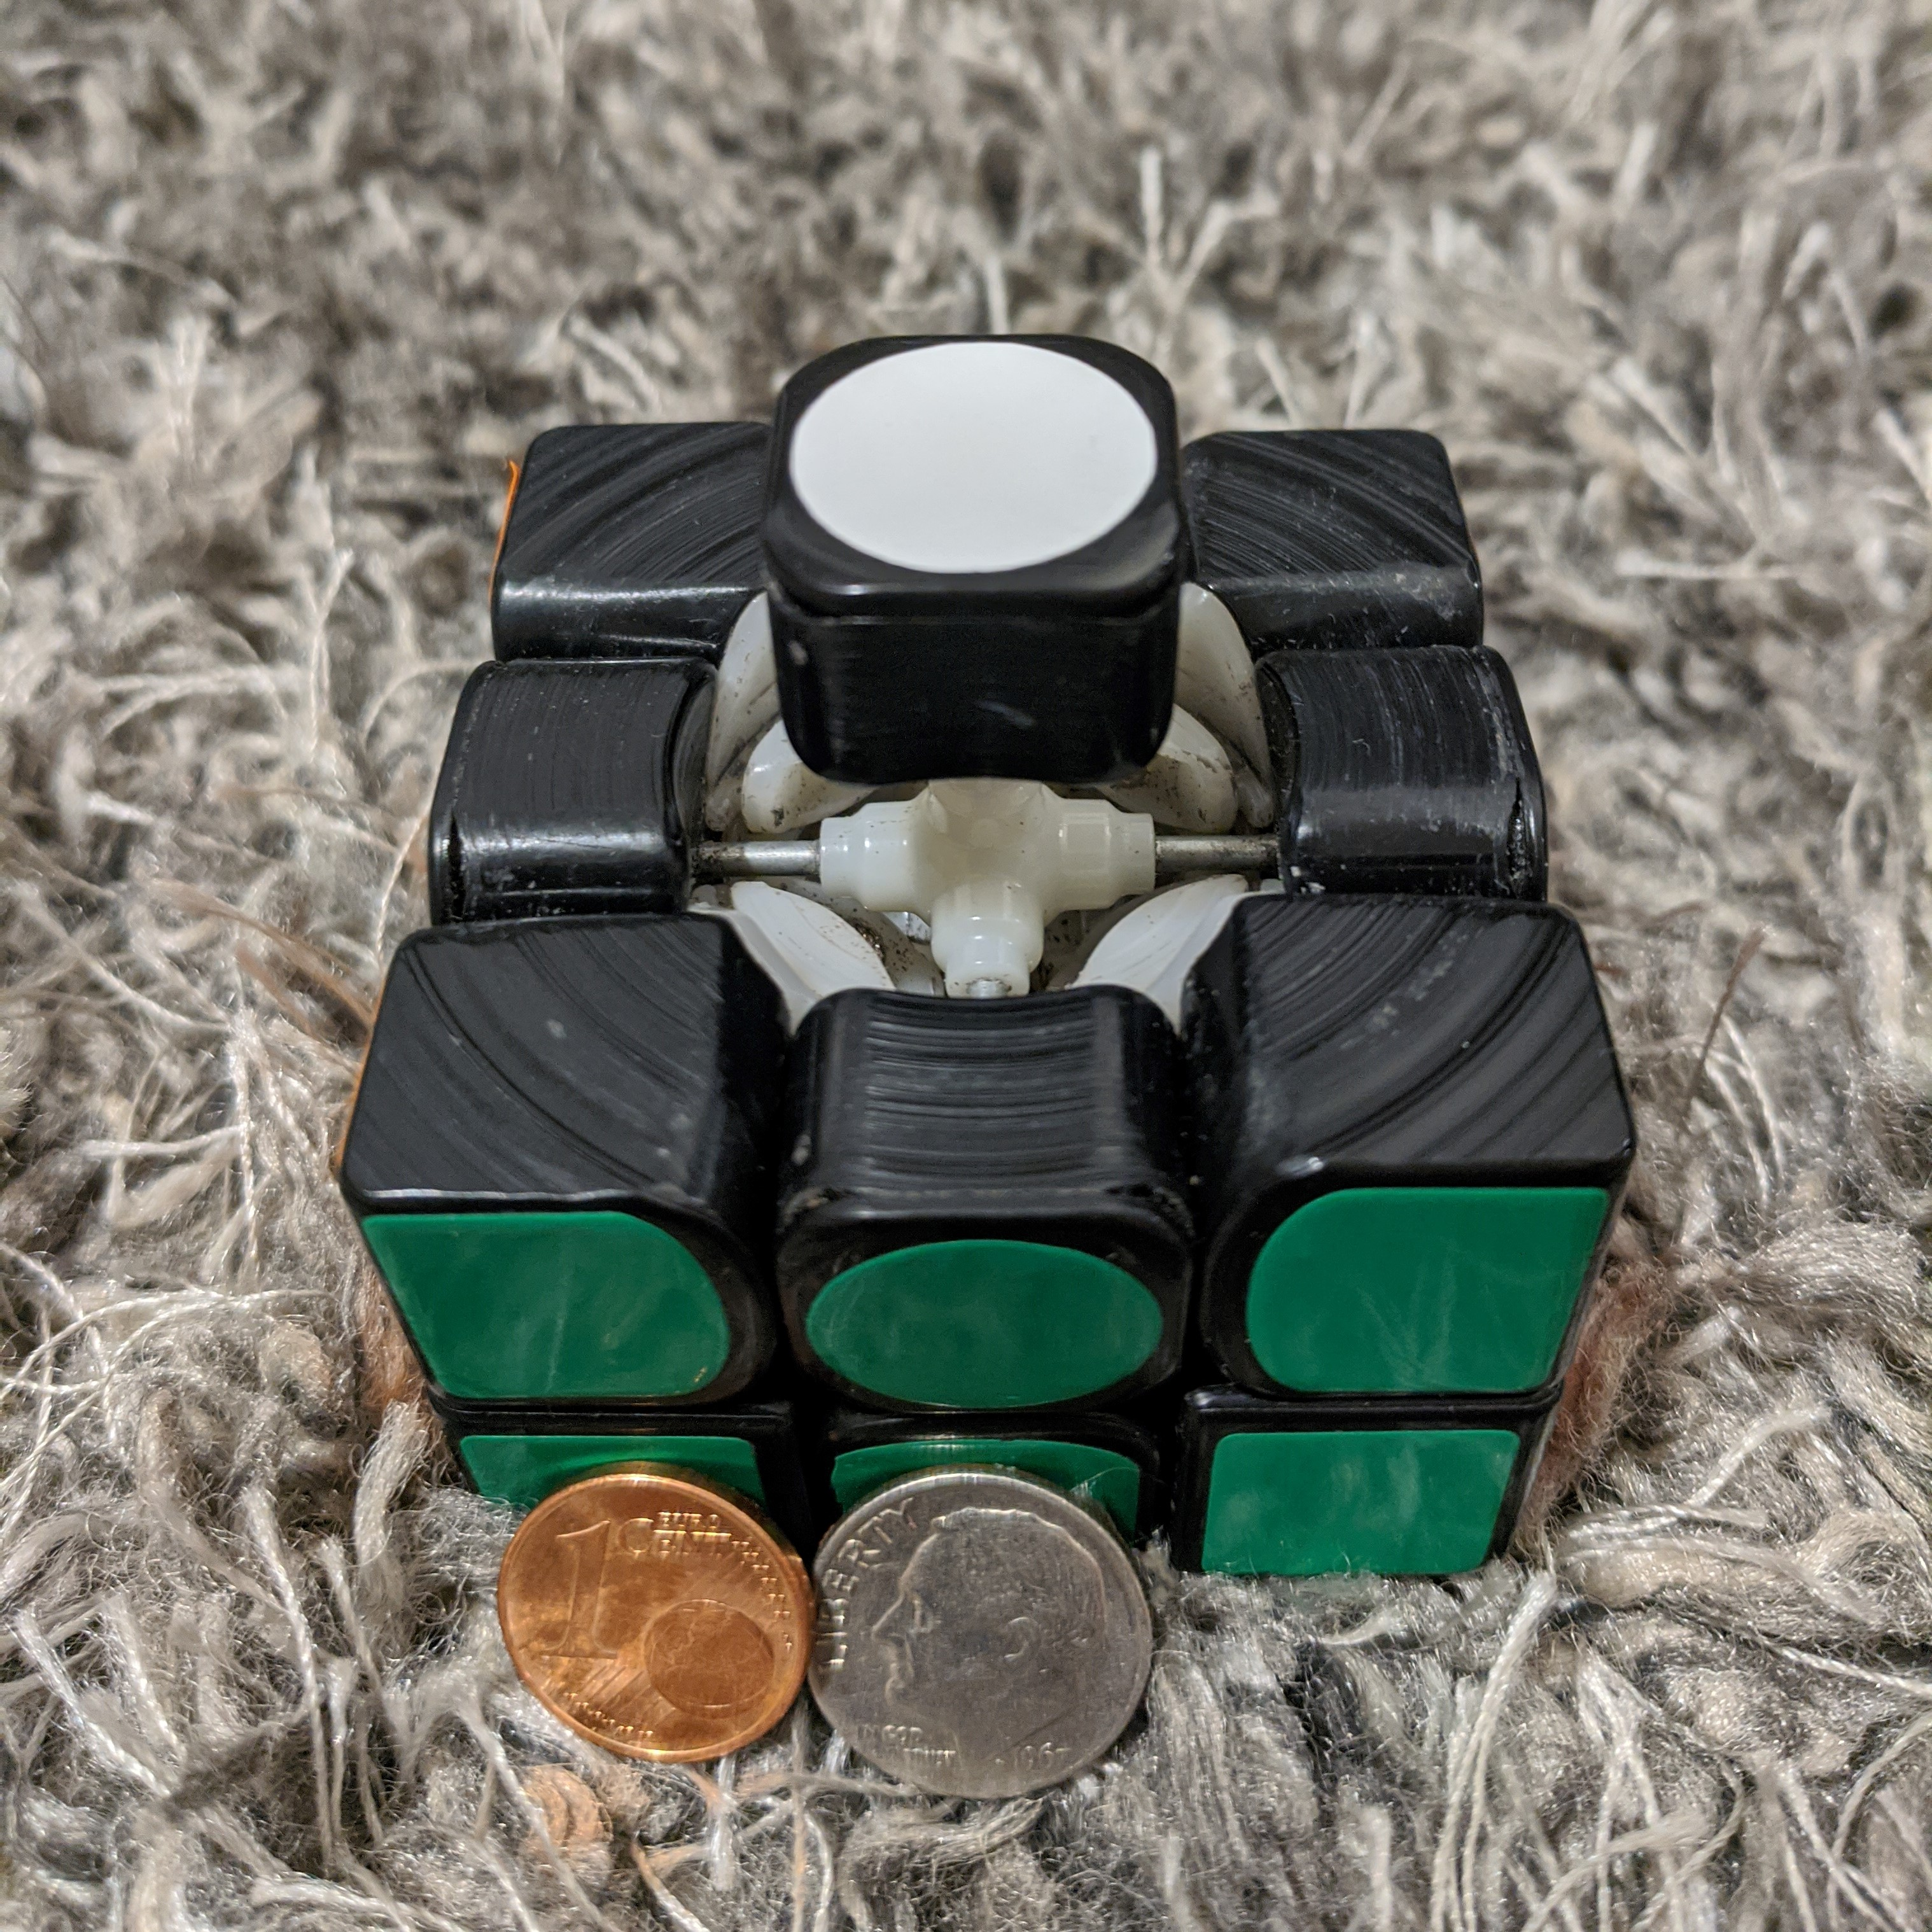
\includegraphics[width=\linewidth]{Figures/6 PCB Design/356_core_cropped.jpg}
    \end{subfigure}
    \begin{subfigure}{.45\textwidth}
        \centering
        \caption{View of the space inside the centerpiece}
        \label{fig:356-core-open}
        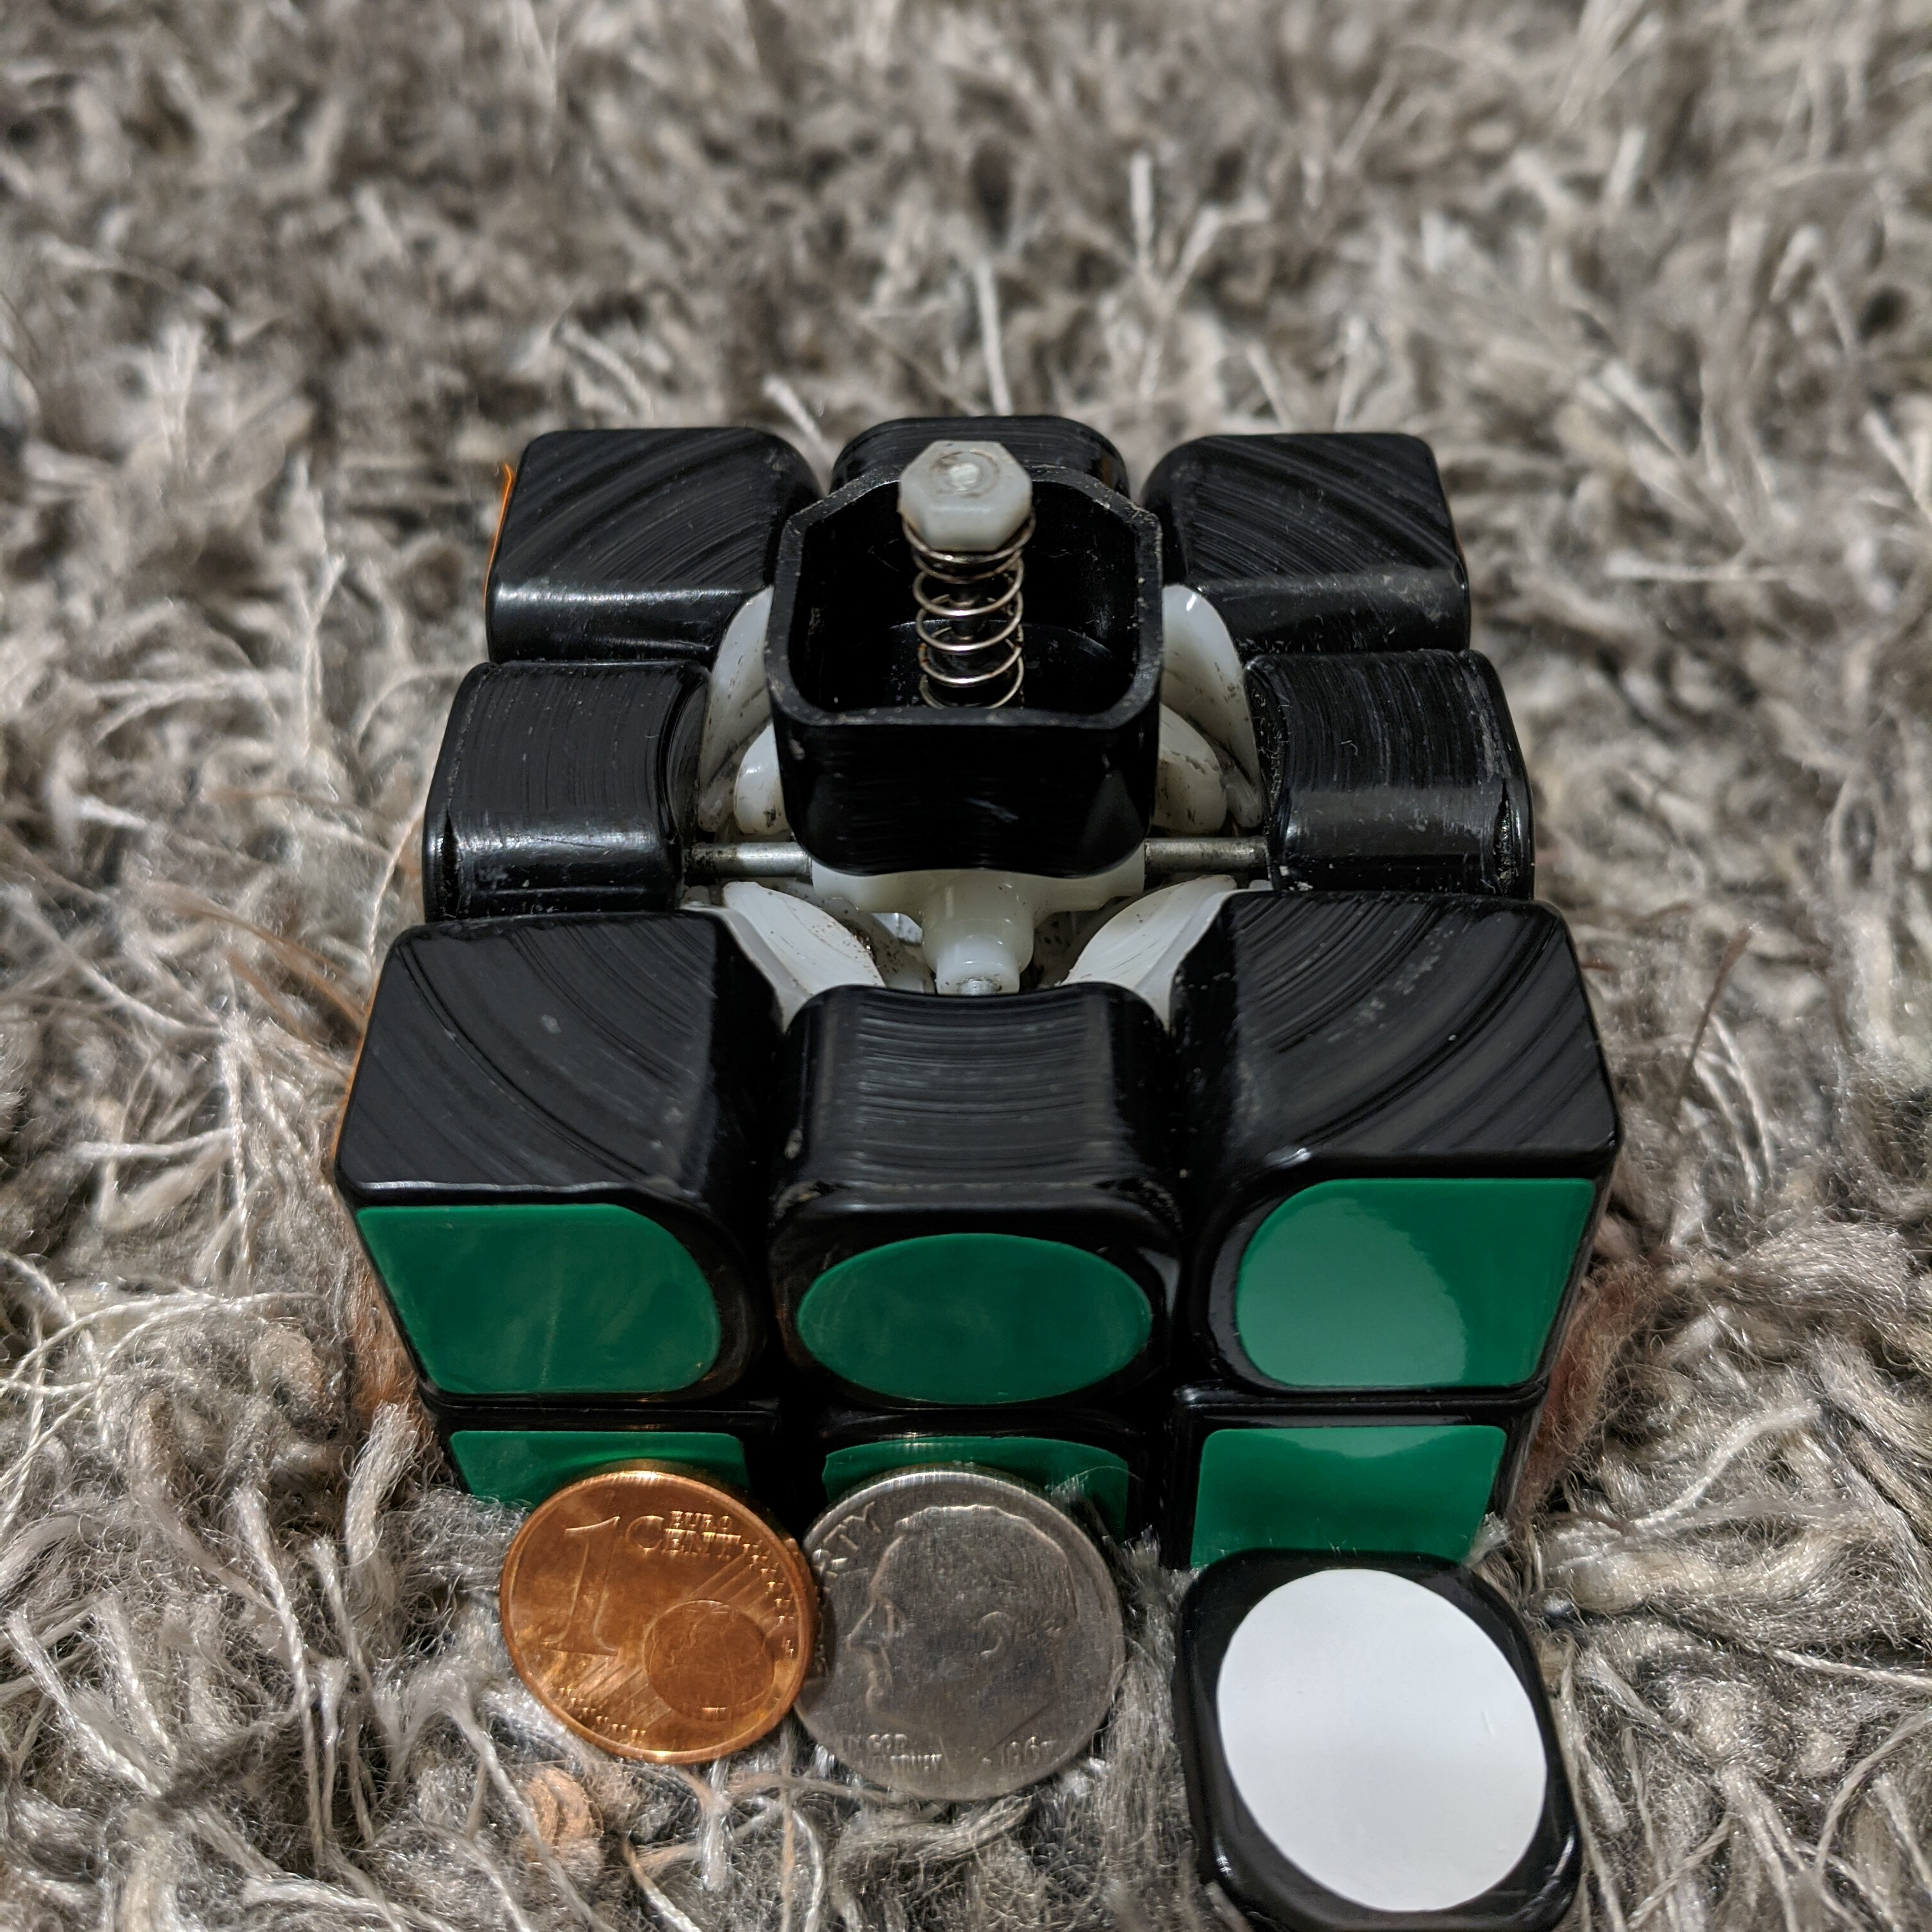
\includegraphics[width=\linewidth]{Figures/6 PCB Design/356_core_open_cropped.jpg}
    \end{subfigure}
\end{figure}


\newpage
\section{Design}
\label{sec:transmitter-design}

Given the above constrains, this section will detail a design for a
printed circuit board capable of precisely generating four distinct
tones (Requirements \ref{subsec:precision-of-tone-generation} and
\ref{subsec:responsiveness-to-face-turns})

\subsection{The 555 Timer}
\label{sec:the-555-timer}

The core component in this PCB design is a 555 timer, which is a
computer chip that facilitates the generation of many types of voltage
frequencies in a circuit.

For this transmitter, the 555 timer will be configured to output a
square wave voltage signal with a 50\% duty cycle (i.e. "Astable
Operation") \cite{icm7555}. This means the voltage on the output pin
will alternate between low and high, spending equal amounts of time in
each state.

The attentive reader will notice that the square wave signal proposed
here differs from the sine wave used to create the synthetic audio in
Figure \ref{fig:code-generate-alg-audio}. Valid concerns may even be
raised about the fact that a square wave is actually a composite of a
fundamental sine wave and infinitely many harmonics \cite{harmonics}.
However, since the nearest harmonic in a square wave with a 50\% duty
cycle oscillates at a frequency three times as fast as the fundamental
\cite{square-waves}, then choosing a fundamental frequency of at least
6.67kHz places the nearest harmonics beyond the range of frequencies
measurable by a typical smartphone or laptop microphone (see Section
\ref{subsec:frequency-response-range}).

The standard schematic for creating this type of voltage signal is
depicted in Figure \ref{fig:555_astable}.

\begin{figure}[h]
    \centering
    \caption{Standard 555 Timer Circuit for Astable Operation \cite{icm7555}}
    \label{fig:555_astable}
    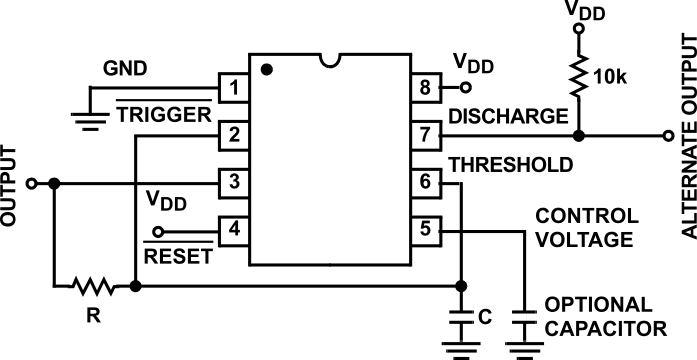
\includegraphics[width=0.75\linewidth]{Figures/6 PCB Design/555_astable.png}
\end{figure}

The two key components are the resistor \code{R} and the capacitor
\code{C} whose respective resistance and capacitance control the output
frequency \code{f} via the relation shown in Equation \ref{eq:555-freq}
\cite{icm7555}:

\begin{equation}\label{eq:555-freq}
    f = \frac{1}{1.4 R C}
\end{equation}

\subsection{Creating Audio}

The 555 timer's varying voltage output can be easily converted to
audible sound by attaching a voltage controlled speaker to the output
wire coming from pin 3 in Figure \ref{fig:555_astable}. However, this
will only produce one continuous tone, and each centerpiece will need
to be able to switch between four distinct tones. As such, the resistor
\code{R} will need to be replaced with four separate resistors (labeled
\code{R1}, \code{R2}, \code{R3}, \code{R4} in Figure
\ref{fig:555_astable_modded}) and a switch. The switch will be
connected to the cube so that a 90$^\circ$ rotation will change which
resistor is in series with the circuit, thus changing the output audio
frequency of the speaker.

\begin{figure}[h]
    \centering
    \caption{Centerpiece State Transmitter Circuit}
    \label{fig:555_astable_modded}
    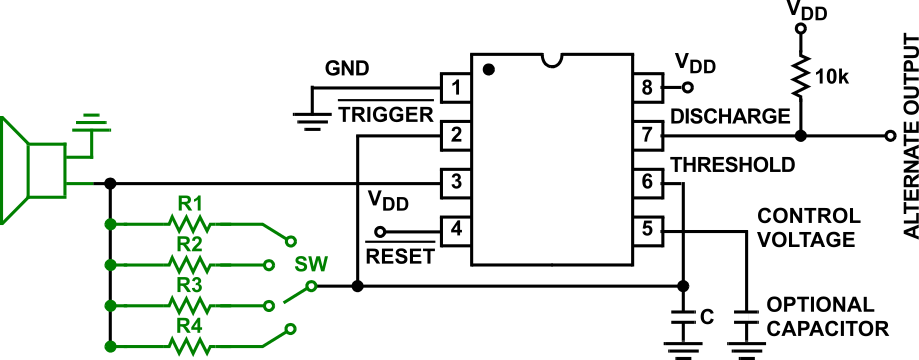
\includegraphics[width=\linewidth]{Figures/6 PCB Design/555_astable_modded.png}
\end{figure}

Alternatively, it is mathematically valid to instead switch between
four different capacitors of different capacitance. However, for the
reasons described in Section \ref{subsec:freq-selection}, opting to
switch between resistors proved more practical.

\subsection{Choosing the values of \code{R} and \code{C}}
\label{subsec:freq-selection}

\begin{sidewaysfigure}
    \centering
    \caption{Output Frequencies of Common \code{R} and \code{C} Values}
    \label{fig:freq-selection}
    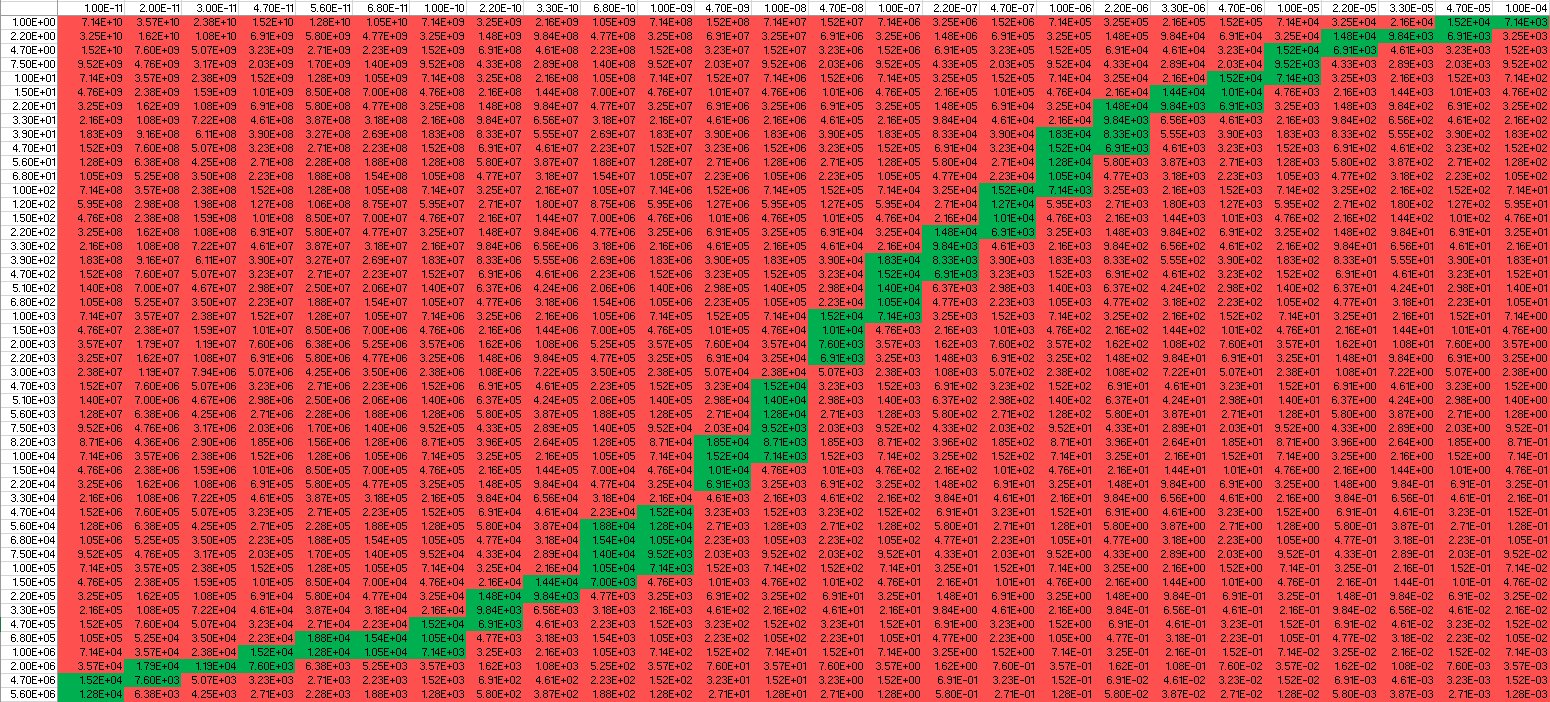
\includegraphics[width=\linewidth]{Figures/6 PCB Design/freq_selection.png}
\end{sidewaysfigure}

There are infinitely many combinations of \code{R} and \code{C} that
will produce any single desired output frequency \code{f}; however, the
set of resistances and capacitances of commonly produced resistors and
capacitors is finite. While multiple components can be combined to
produce more specific resistances and capacitances, doing so would
increase the overall component count for a circuit board that is
constrained to a small physical size. As such, this proof-of-concept
design will focus on producing frequencies attainable with a single
capacitor and resistor pair.

Since each centerpiece transmitter needs to produce four distinct
frequencies, four separate capacitor-resistor pairs are required.
However, since the output frequency can be varied by adjustments to
\emph{either} the capacitance \emph{or} resistance, one of those two
options can be held constant to reduce the overall component count.

To chose which one to hold constant, the output frequencies of all
possible pairings of capacitors and resistors from two cheap Amazon
kits \cite{amazon-capacitors} \cite{amazon-resistors} were calculated
using Equation \ref{eq:555-freq}. The resulting table was then color
coded to highlight the usable frequencies in green (6.67kHz to
20kHz)\footnote{6.67kHz is the lower bound derived in Section
\ref{sec:the-555-timer} and 20kHz the upper limit of the typical
frequency response range discussed in Section
\ref{subsec:frequency-response-range}} while leaving all other unusable
frequencies in red. The result is shown in Figure
\ref{fig:freq-selection} with the various resistances shown on the
vertical axis and the various capacitances along the horizontal axis.

A close observation of the resulting sigmoid shape of usable
frequencies reveals only one location where there are at least four
usable frequencies associated with a fixed resistance (i.e. row of
green cells), compared to ten locations where there are at least four
usable frequencies associated with a fixed capacitance (i.e. column of
green cells). As such, the most practical value to hold constant here
is the capacitance.

One of the locations with a viable fixed capacitance is shown in Figure
\ref{fig:freq-selection-r}. This pairing of a 10nF capacitor with four
resistors with respective resistances of 4.7k$\Omega$, 5.1k$\Omega$,
5.6k$\Omega$, and 7.5k$\Omega$ will be used in the prototype created in
Section \ref{sec:prototype}.

\begin{figure}[h]
    \centering
    \caption{Output Frequencies of Common \code{R} and \code{C} Values}
    \label{fig:freq-selection-r}
    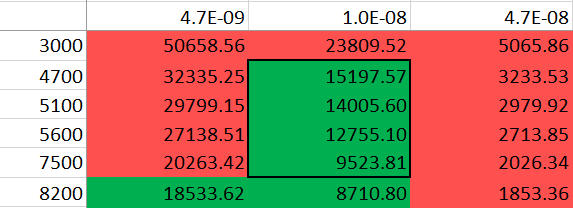
\includegraphics[width=0.75\linewidth]{Figures/6 PCB Design/freq_selection_r.png}
\end{figure}


\section{Prototyping}
\label{sec:prototype}

The key step to produce a proof-of-concept for Requirements
\ref{subsec:precision-of-tone-generation} and
\ref{subsec:responsiveness-to-face-turns} is to put everything together
on a breadboard and turn on the power while recording the output audio
to make sure four distinct tones are produced.

This step begins by gathering all the components from the schematic in
Figure \ref{fig:555_astable_modded} with the specific values of
\code{C}, \code{R1}, \code{R2}, \code{R3}, and \code{R4} shown in
Figure \ref{fig:freq-selection-r}. These components are then placed
onto a physical breadboard in accordance with the schematic's defined
layout. Connecting \code{VDD} and \code{GND} to power then causes the
speaker to produce a tone. With power still connected, the switch can
be moved to put any other resistor in series to change the resulting
tone of the speaker.

The result is shown in Figure \ref{fig:breadboard}. The left section of
the figure shows a spectrogram of the four distinct tones produced by
moving the green wire (representing the rotary switch) through each of
the four resistors on the breadboard in the right section of the figure.

\begin{figure}
    \centering
    \caption{Breadboard Prototype}
    \label{fig:breadboard}
    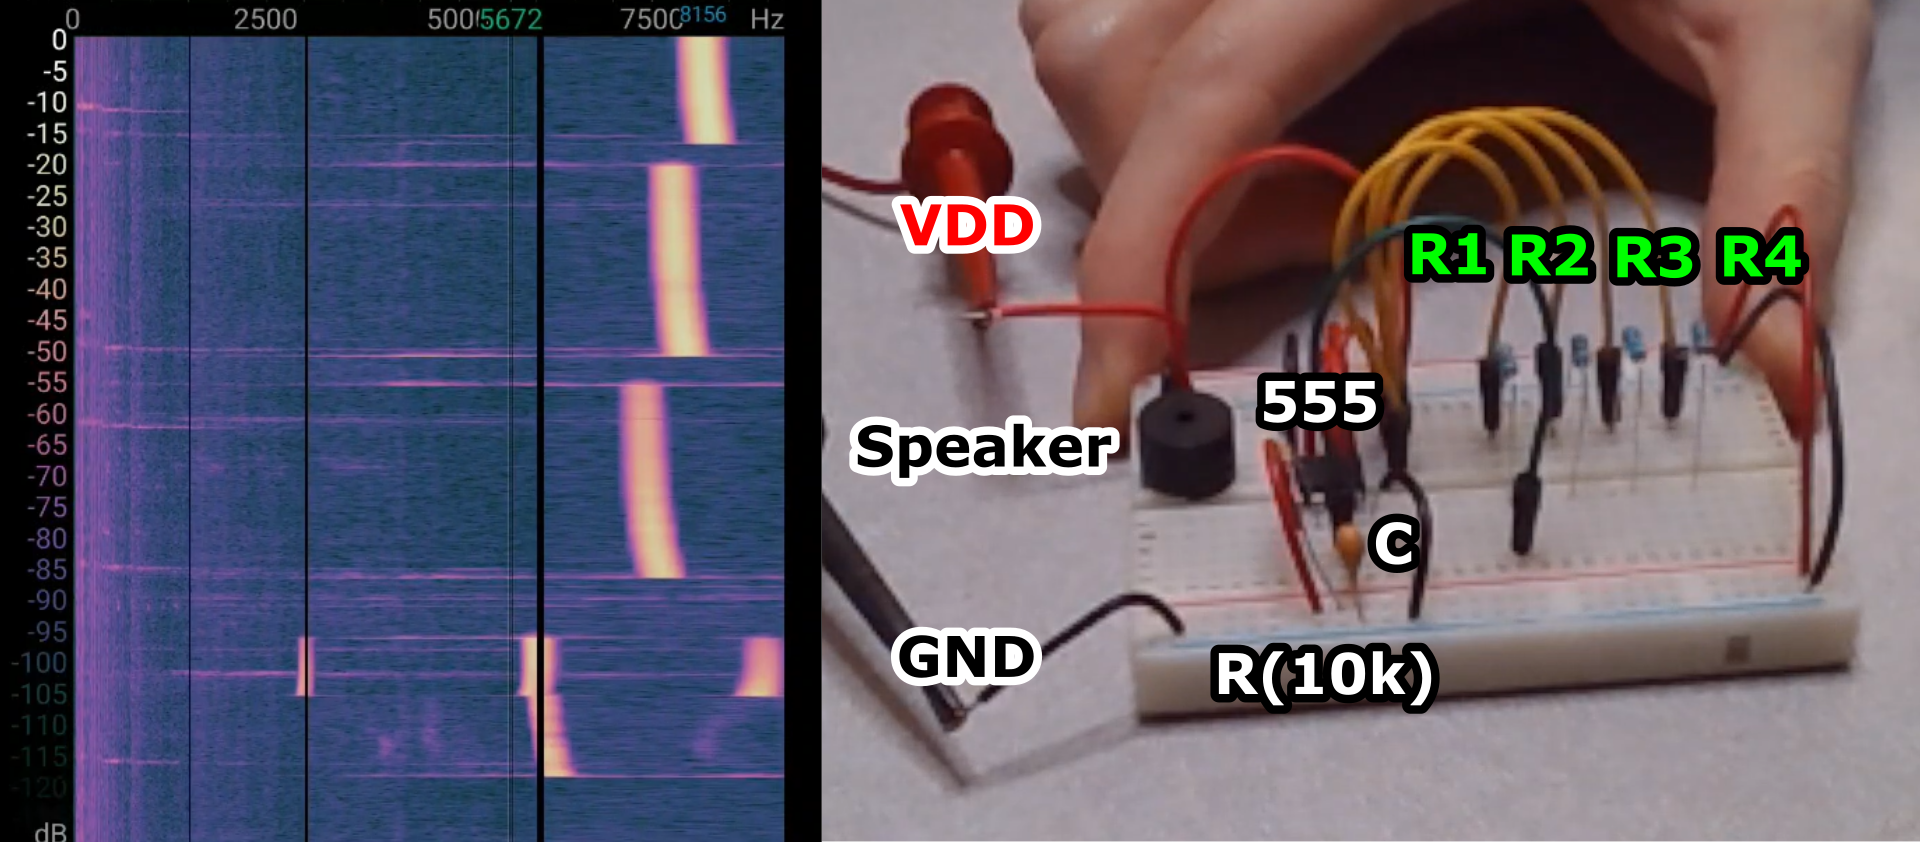
\includegraphics[width=\linewidth]{Figures/6 PCB Design/breadboard_spectrogram.png}
\end{figure}


\section{Minimizing Sound Obstruction}
\label{sec:minimizing-sound-obstruction}

\begin{figure}
    \centering
    \caption{Effects of Various Sound Obstructions on Signal Intensity}
    \label{fig:obstruction}
    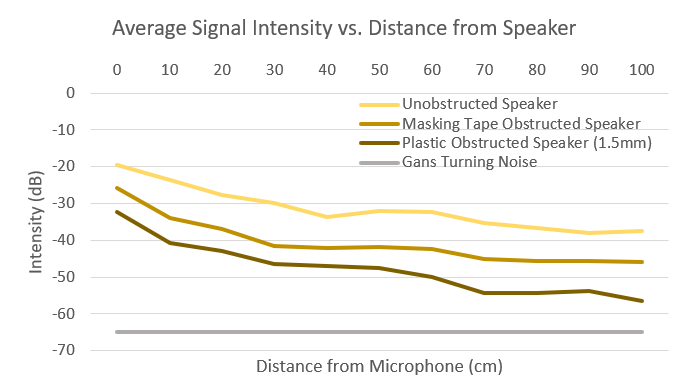
\includegraphics[width=\linewidth]{Figures/6 PCB Design/obstruction_intensity.png}
\end{figure}

In preparation for miniaturizing the prototype circuit from Section
\ref{sec:prototype} to fit inside a speedcube's centercap, an
experiment was performed to measure the effects of various physical
barriers on the signal-to-noise ratio of a small speaker against
background noise created by solving a Gans 356 speedcube (Requirement
\ref{subsec:transmitter-signal-to-noise-ratio}).

Specifically, three different types of obstructions were placed between
a speaker similar to the type that would fit inside a speedcube
centercap and a phone microphone: no obstruction, a piece of masking
tape over the speaker (representative of a sticker on a speedcube), and
a full plastic enclosure of the same thickness as a speedcube
centercap. For each of these obstructions, the source speaker emitted
eight different tones across the human audible spectrum and the average
intensity of the signal was measured with the microphone at 10cm
increments up to a full meter away from the speaker.

Figure \ref{fig:obstruction} shows the resulting signal strength for
each obstruction type (the top three yellow lines) compared with the
background noise caused by solving a Gans 356 speedcube (the bottom
gray line). As expected, the signal strength tapered off for all three
obstruction types as the microphone moved farther away from the signal,
and larger obstructions reduced the signal strength more than smaller
obstructions.

Of most interest are the signal intensities between 10cm and 30cm from
the microphone since that's the typical distance between a speedcuber's
cube and his/her smartphone or laptop while practicing at home. By the
far end of that range, only the completely unobstructed speaker's
signal stayed above the -30dB limit discussed in Section
\ref{subsubsec:key-observations-from-the-spectrogram}. As such, it is
clear that successfully miniaturizing the prototype circuit to fit
inside a centercap will require a custom centercap design with space
for sound to exit unobstructed and/or a speaker significantly louder
than the ones used in these prototypes.

As a tangential note, the fact that the unobstructed speaker's signal
strength drops to nearly -40dB at only 100cm away from the speaker
means that the cube's moves cannot be reliably tracked while the cube
is at a distance from the receiving microphone. This property may prove
beneficial for competitive environments as a potential path towards
allowing automated move tracking during competitive solves without
incurring the risks of competitors using smartcubes as a way to spy on
the scrambling process for an unfair advantage.


\section{Miniaturization}
\label{sec:miniaturization}

Finally, to address Requirement
\ref{subsec:prospects-of-miniaturization}, this section will
demonstrate that all the required components can fit within the limited
16mm$^2$ of space inside a single center cap of a Gans 356 Speedcube.

Meeting this size constraint is best achieved by swapping out the large
through-hole resistors, capacitors, and 555 timer used in the prototype
for smaller surface mount (SMD) components. Additionally, the large
black buzzer can be swapped out for a much thinner piezo buzzer that
can lay on flat on top of a custom-designed replacement centercap.
Finally, the DC power supply can be changed out for a button-cell
battery oriented vertically.

An example of the final result could look like Figure
\ref{fig:core-placement}. Notice that all required components easily
fit inside of a custom designed center cap that fits perfectly into a
Gans 356 speedcube without inhibiting the cube's freedom of rotation.
Also notice the large hole in the center of the custom centercap
visible in Figure \ref{fig:core-circuit} that provides an unobstructed
path for the speaker's signal to exit the center cap.

The one required component not shown in Figure \ref{fig:core-placement}
is the rotary switch required to change the resistor actively in series
with the circuit. This particular component could be modeled after the
rotary switches placed on the reverse sides of the PCBs embedded within
the centercaps of the commerical smartcubes shown in Section
\ref{sec:commercial-smartcubes}.

\begin{figure}[h]
    \centering
    \caption{Transmitter Circuit Inside a Custom Gans 356 Centercap}
    \label{fig:core-placement}
    \begin{subfigure}{.30\textwidth}
        \centering
        \caption{Internal View}
        \label{fig:core-circuit}
        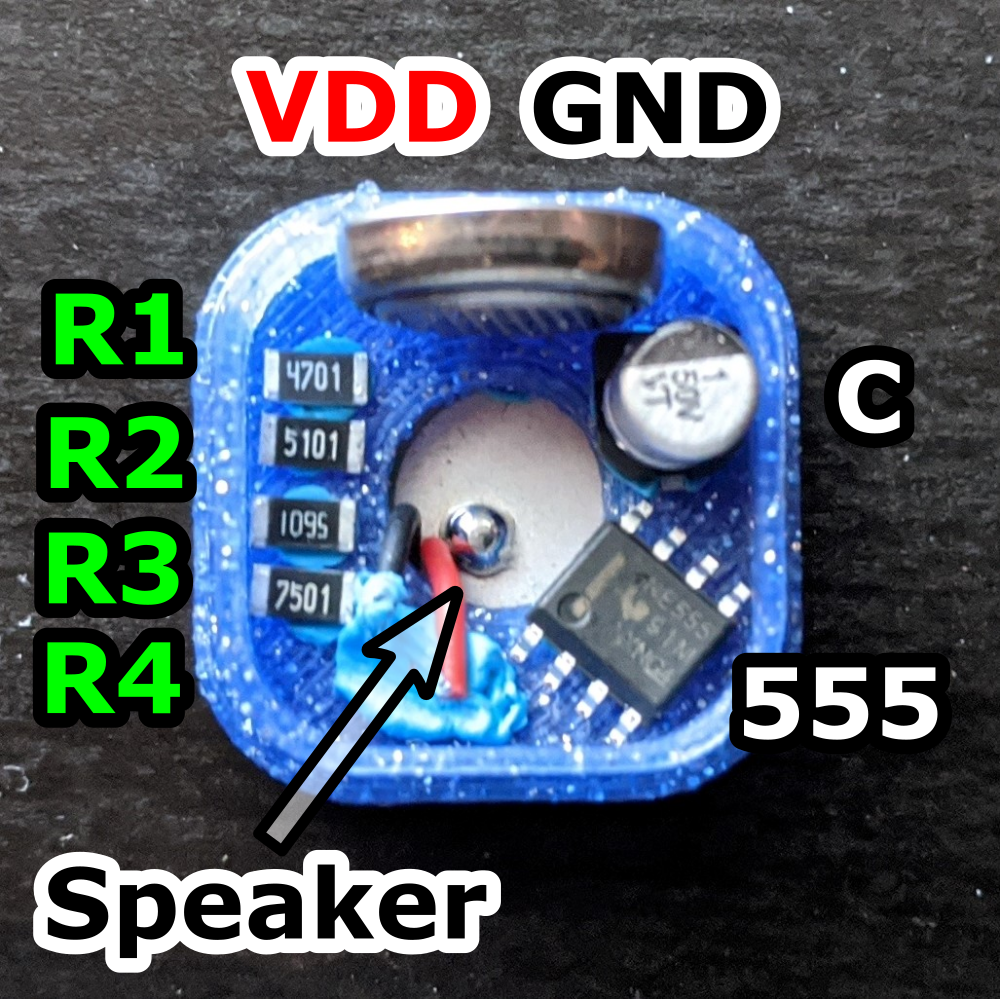
\includegraphics[width=\linewidth]{Figures/6 PCB Design/core_labelled.png}
    \end{subfigure}
    \begin{subfigure}{.30\textwidth}
        \centering
        \caption{Bird's Eye View}
        \label{fig:core-placement-birds-eye}
        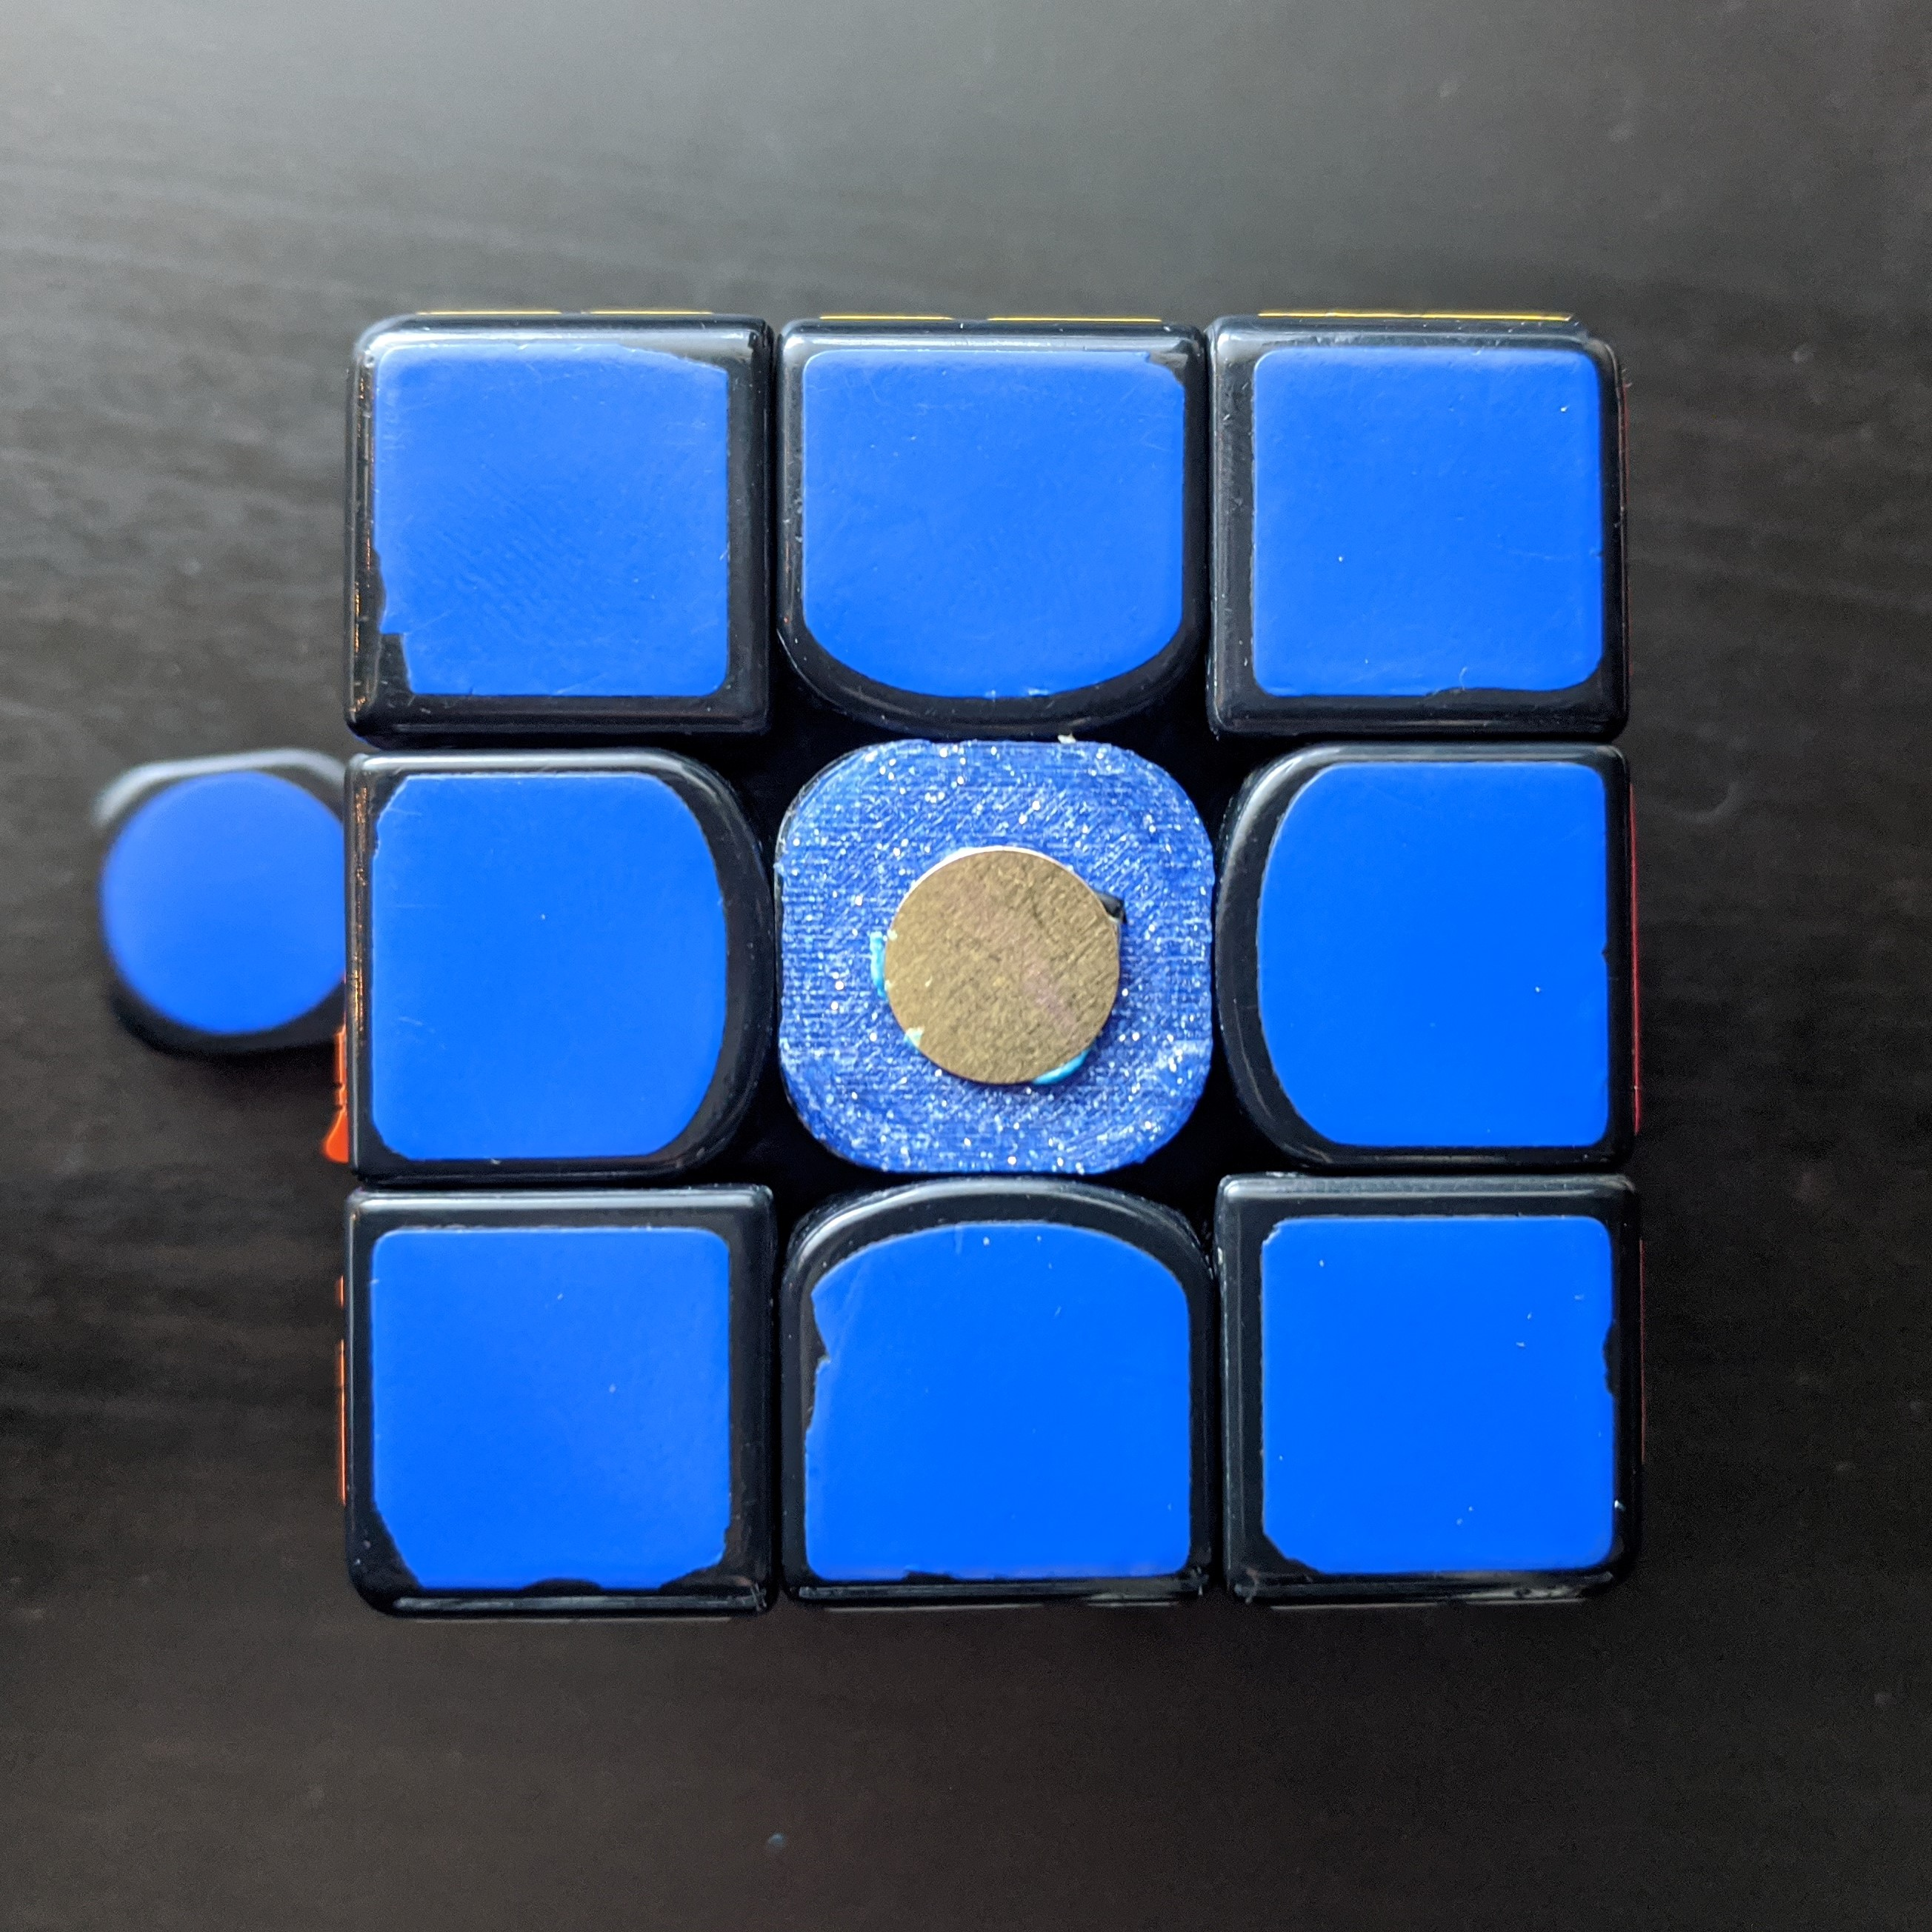
\includegraphics[width=\linewidth]{Figures/6 PCB Design/core_placement_birds_eye_square.jpg}
    \end{subfigure}
    \begin{subfigure}{.30\textwidth}
        \centering
        \caption{Isometric View}
        \label{fig:core-placement-isometric}
        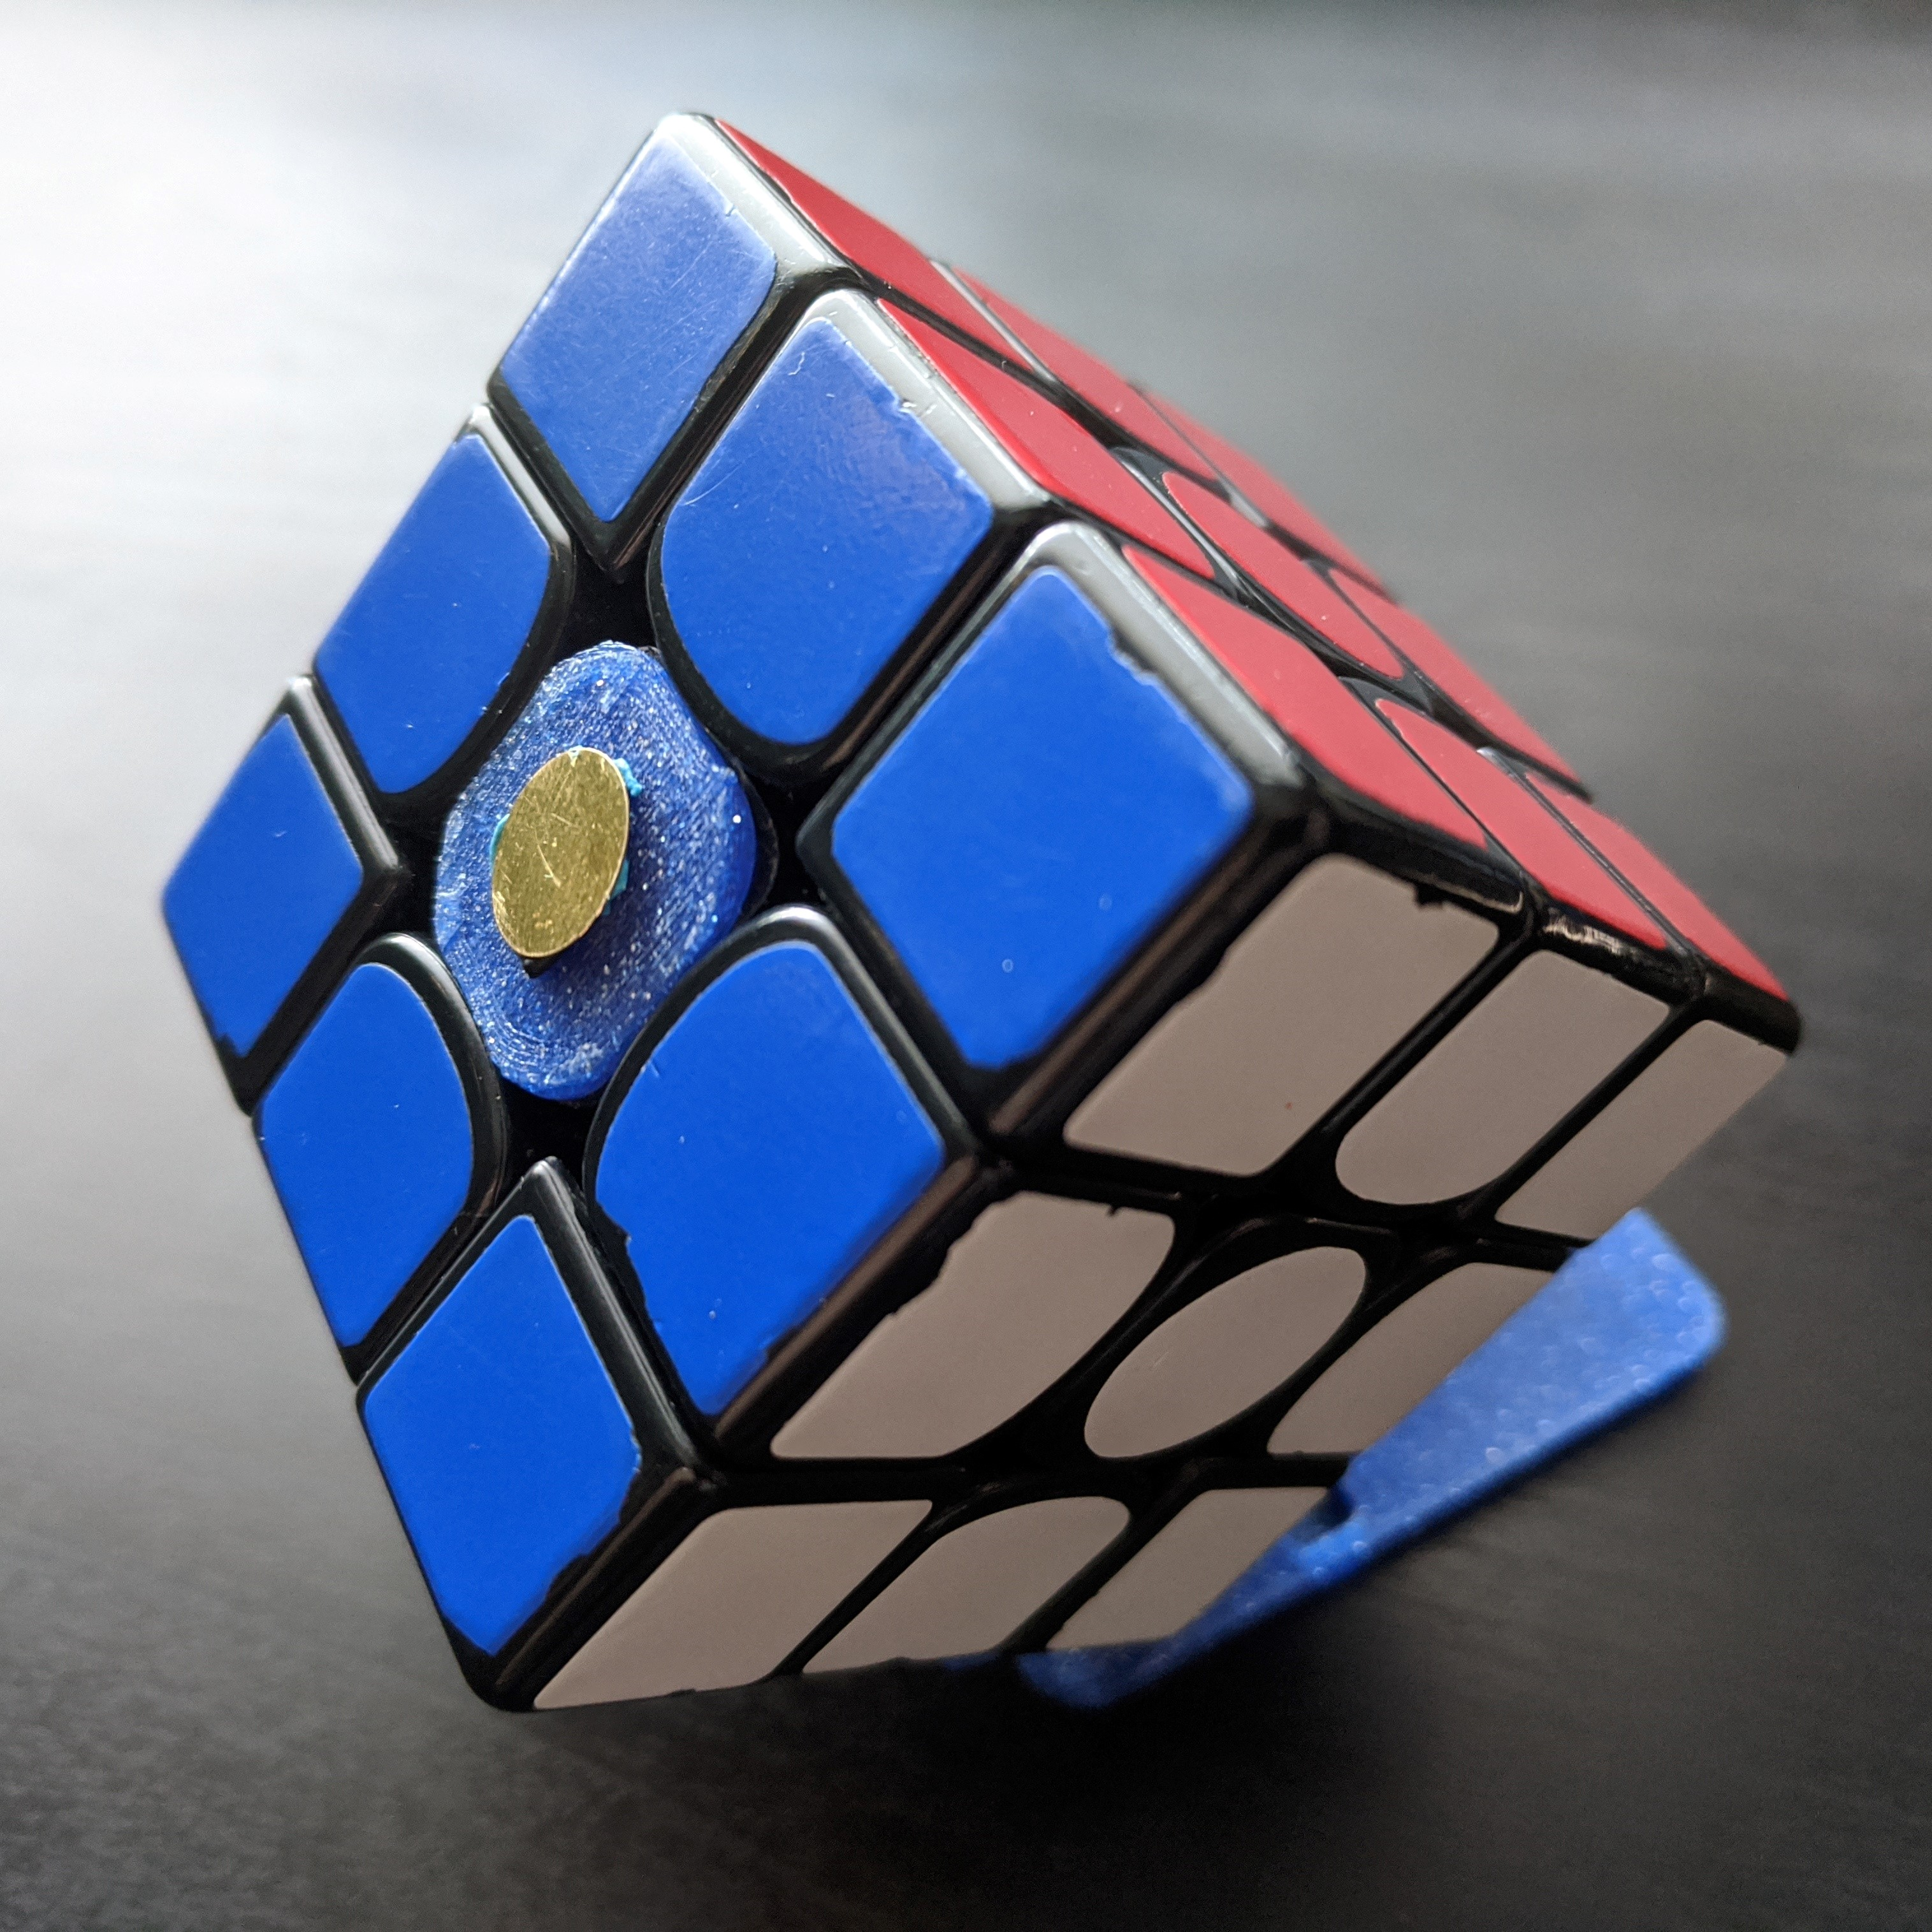
\includegraphics[width=\linewidth]{Figures/6 PCB Design/core_placement_isometric_square.jpg}
    \end{subfigure}
\end{figure}


\section{Summary}

In summary, this chapter demonstrated a proof of concept for a PCB
capable of transmitting the current state of a Rubik's Cube via sound
to the receiver described in Chapter \ref{Chapter5}. This
proof-of-concept circuit works by using specific capacitors and
resistors to produce a precise voltage frequency from a 555 timer that
can be output into the audible spectrum by connecting a speaker. In
addition to showing a working circuit on a breadboard, this chapter
also described the results of an experiment showing the need for an
unobstructed path between the transmitter and the receiver. Finally,
this chapter showed how all the required components for the transmitter
could reasonably fit inside a single centercap of a speedcube like the
Gans 356.

Future researchers could build on the work of this chapter by
engineering more refined prototypes to more completely validate if this
proposed design is capable of meeting requirements
\ref{subsec:responsiveness-to-face-turns},
\ref{subsec:transmitter-signal-to-noise-ratio}, and
\ref{subsec:prospects-of-miniaturization}. Such refinements could start
with a rotary encoder and/or fully miniaturizing the PCB and actuating
the frequency change with the speedcube's rotation.
